\documentclass[fleqn,10pt]{SelfArx}
\usepackage[english]{babel}
\usepackage{lipsum}
\usepackage{url}
\usepackage{balance}

\newcommand{\code}[1]  {\texttt{\footnotesize{#1}}}
\newcommand{\lin}[1]{(\emph{ln. #1}\xspace)}
\newcommand{\linx}[1]{\emph{ln. #1}\xspace}

\usepackage{xspace}
\usepackage{hyperref}
\usepackage{mathptmx}
\usepackage{graphicx}
\usepackage{times}
\usepackage{textcomp}
\usepackage{gensymb} % degree. ie 360º
\usepackage{amsmath}
\usepackage{comment}
\usepackage{multirow}
\usepackage[framemethod=tikz]{mdframed}
\usepackage{graphicx}
\usepackage[labelfont=bf]{subcaption}

\usepackage{tcolorbox}% http://ctan.org/pkg/tcolorbox
\definecolor{mycolor}{rgb}{0,0,0}% Rule colour
\makeatletter
\newcommand{\mybox}[1]{%
	\setbox0=\hbox{#1}%
	\setlength{\@tempdima}{\dimexpr\wd0+13pt}%
	\begin{tcolorbox}[colframe=mycolor,boxrule=0.5pt,arc=4pt,
		left=6pt,right=6pt,top=6pt,bottom=6pt,boxsep=0pt,width=\@tempdima]
		#1
	\end{tcolorbox}
}
\makeatother
\usepackage[resetlabels,labeled]{multibib}
\newcites{A}{Appendix}
\usepackage[num]{abntex2cite}
\citebrackets[]
%----------------------------------------------------------------------------------------
%	COLUMNS
%----------------------------------------------------------------------------------------
\setlength{\columnsep}{0.55cm} % Distance between the two columns of text
\setlength{\fboxrule}{0.75pt} % Width of the border around the abstract
%----------------------------------------------------------------------------------------
%	COLORS
%----------------------------------------------------------------------------------------
\definecolor{color1}{RGB}{0,0,90}
\definecolor{color2}{RGB}{0,20,20}
%----------------------------------------------------------------------------------------
%	HYPERLINKS
%----------------------------------------------------------------------------------------
\usepackage{hyperref} % Required for hyperlinks
\hypersetup{hidelinks,colorlinks,breaklinks=true,urlcolor=color2,citecolor=color1,linkcolor=color1,bookmarksopen=false,pdftitle={Title},pdfauthor={Author}}
%----------------------------------------------------------------------------------------
%	ARTICLE INFORMATION
%----------------------------------------------------------------------------------------
\JournalInfo{\color{gray}\normalsize\sffamily\bfseries Revista de Informática Teórica e Aplicada - RITA - ISSN 2175-2745\\ Vol.~XX, Num.~XX~(2018)~11-XX} % Journal information
\Archive{\mybox{RESEARCH ARTICLE}} % Type of Article: Researh, Review, Tutorial, Study Case

\PaperTitle{Symmetric Peer-to-Peer Applications}
\ShortTitle{Symmetric Peer-to-Peer Applications}

\Titulo{Aplicações Peer-to-Peer Simétricas}

\PaperVol{XX} % Volume 
\PaperNum{X} % Number 
\PaperAno{YYYY} % Year of Publication

\Authors{Francisco Sant'Anna\textsuperscript{1}*}
\affiliation{\textsuperscript{1}\textit{Department of Computer Science, Rio de Janeiro State University (UERJ), Brazil}}
\affiliation{*\textbf{Corresponding author}: francisco@ime.uerj.br}

\Keywords{collaboration --- determinism --- peer-to-peer --- time machine }

\newcommand{\keywordname}{Keywords} % Defines the keywords heading name

\PalavrasChave{colaboração --- determinismo --- peer-to-peer --- máquina do tempo} 
\Doi{http://dx.doi.org/10.22456/2175-2745.XXXX} % DOI
\DateR{dd/mm/yyyy} % Received
\DateA{dd/mm/yyyy} % Accepted

%----------------------------------------------------------------------------------------
%	ABSTRACT
%----------------------------------------------------------------------------------------

\Abstract{
In real-time networked applications, such as shared documents, users can
interact remotely and yet share the exact same experience as if they were in a
single machine.
%
In this work, we propose a middleware for \emph{symmetric peer-to-peer
applications} in which decentralized instances can trigger asynchronous events
and yet conform to identical behavior.
%
Peers are allowed to join and leave the network at any time.
Application developers must adhere to a restricted API, which is deterministic,
stateless, and only supports pre-allocated memory.
%
The middleware is responsible for synchronizing the events in a global shared
timeline across the network.
Also, based on memory snapshots and deterministic simulation, a ``time machine''
can rollback conflicting peers to resynchronize their state.
%
We show that the middleware can handle applications with over 20 peers in a
heterogeneous topology under high churn.
For instance, in a simulation scenario of 25 events per minute with a network
latency of 50ms, the peers need to roll back and resynchronize only 3\% of
the time.
}

\Resumo{
Em aplicações de tempo real em rede, tais como documentos compartilhados, os
usuários podem interagir remotamente e ainda obterem a mesma experiência, como
se estivessem em uma única máquina.
%
Neste trabalho, nós propomos um middleware para \emph{aplicações peer-to-peer
simétricas} nas quais instâncias descentralizadas podem disparar eventos
assíncronos e ainda obterem comportamento idêntico.
%
Os pares podem entrar e sair da rede a qualquer momento.
Os desenvoledores de aplicações devem aderir a uma API restritiva, que deve ser
determinística, sem estados internos, e também com alocação prévia de memória.
%
O middleware é responsável por sincronizar os eventos em uma linha de tempo
global e compartilhada em toda a rede.
Além disso, com base em cópias da memória e simulação determinística, uma
``máquina do tempo'' pode retroceder pares em conflito para ressincronizar o
seu estado.
%
Nós mostramos que o middleware suporta aplicações com mais de 20 pares em uma
topologia heterogênea e sob alta taxa de desconexões.
Como exemplo, em uma simulação com 25 eventos por segundo em uma rede com
latência de 50ms, os pares precisam retroceder e ressincronizar somente 3\% do
tempo.
}

%----------------------------------------------------------------------------------------

\begin{document}

%\setcounter{page}{11}

\flushbottom % Makes all text pages the same height
\maketitle % Print the title and abstract box
\thispagestyle{empty} % Removes page numbering from the first page
%\tableofcontents % Print the contents section

\section{Introduction} % The \section*{} command stops section numbering
\label{sec.introduction}

Real-time networked applications allow multiple users to interact remotely and
yet share the same experience.
Examples of these \emph{symmetric distributed applications}~\cite{gals} are
shared documents, watch parties, and multi-player games.
%
In order to reproduce the exact behavior in multiple devices, the application
must be able to synchronize time and execution across the network.
In addition, since users can interact asynchronously with the application,
event occurrences must somehow be synchronized back across devices.

A common approach towards symmetric applications is to introduce a middleware
to orchestrate events and time in the network~\cite{gals,croquet}.
This way, applications developers can rely on middleware primitives to trigger
events, which are intercepted and synchronized in a global shared timeline
across the network.
Developers must also restrict themselves to deterministic and stateless calls
only, such that execution can be equally reproduced in all nodes according to
the shared timeline.
However, current solutions depend on a central server to interconnect network
nodes and determine a shared timeline.

In this work, we propose \emph{symmetric peer-to-peer applications}, which
do not rely on central servers for coordination.
Peers in the application form a dynamic network graph and communicate only
with direct neighbours, as in typical unstructured peer-to-peer
networks~\cite{p2p.survey}.
Events are flooded in the graph and are triggered locally with a small delay
to compensate the network latency.
To deal with events received out of order or too late, a time machine can
rollback peers locally to a previous state and reapply events in order and
in time.
Our main contribution is the design of a middleware to ensure that all peers
    (a) meet event deadlines,
    (b) advance in sync in real time, and
    (c) can leave and join the network and remain symmetric.
We target small peer-to-peer networks, in which nodes are only a few hops away
from each other.
This ensures that events can span the whole network in a reasonable time to
preserve the real-time behavior of applications.
We also assume that peers are non-malicious in the sense that they do not
generate erroneous events.

We perform simulations with over 20 peers in a 5-hop mixed topology with cycles
and straight lines.
We vary the network latency and peer churn, as well as the frequency and
deadlines of events.
%
We then measure (a) the recurrence of time travels, (b) the real-time pace of
peers, and (c) the recoverability from churns, such that they validate our
goals above, respectively.
%
As results, we show that the last two goals are met even under extreme
conditions: peers exhibit a time mismatch of under $0.2\%$ and take less than
$1.5s$ to recover from churns.
%
For the first goal, we identify the scenarios in which the middleware can meet
event deadlines with the desired performance.
As an example, in a scenario of 25 events per minute with a network latency of
$50ms$, the peers need to roll back only $3\%$ of the time.

In Section~\ref{sec.related}, we revisit existing solutions for symmetric
distributed applications and software time machines.
In Section~\ref{sec.tml}, we detail the architecture of our middleware, its
programming API, and how it orchestrates peers.
%In Section~\ref{sec.app}, ...
In Section~\ref{sec.eval}, we evaluate our design under a number of scenarios.
In Section~\ref{sec.conclusion}, we conclude this work.

\section{Related Work}
\label{sec.related}

This section first revisits existing solutions for symmetric distributed
applications, namely Croquet~\cite{croquet,croquet.new}, GALS~\cite{gals}, and
CRDTs~\cite{crdts}.
Then, we discuss software time machines that are built for either local or
networked applications.

\subsection{Symmetric Distributed Applications}
\label{sec.related.sym}

% docs.google.com/spreadsheets/d/1CpMmEgabJq2XQeTDW_BNCV4JWrcMlELuaEjDtw7kwg0/
\begin{figure}
  \centering
  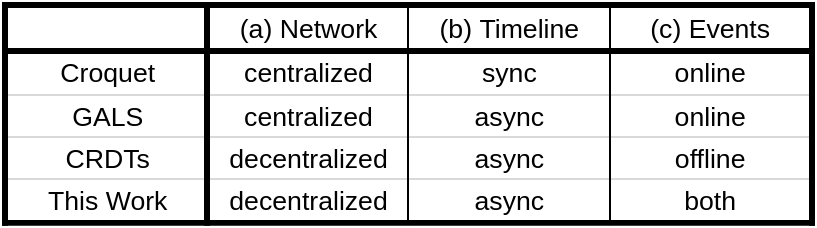
\includegraphics[width=\linewidth]{table}
  \caption{
    Related work regarding
        (a) how the network is organized,
        (b) how global time is determined, and
        (c) how events are propagated and applied.
    \label{fig.table}
  }
\end{figure}

\begin{figure*}
  \centering
  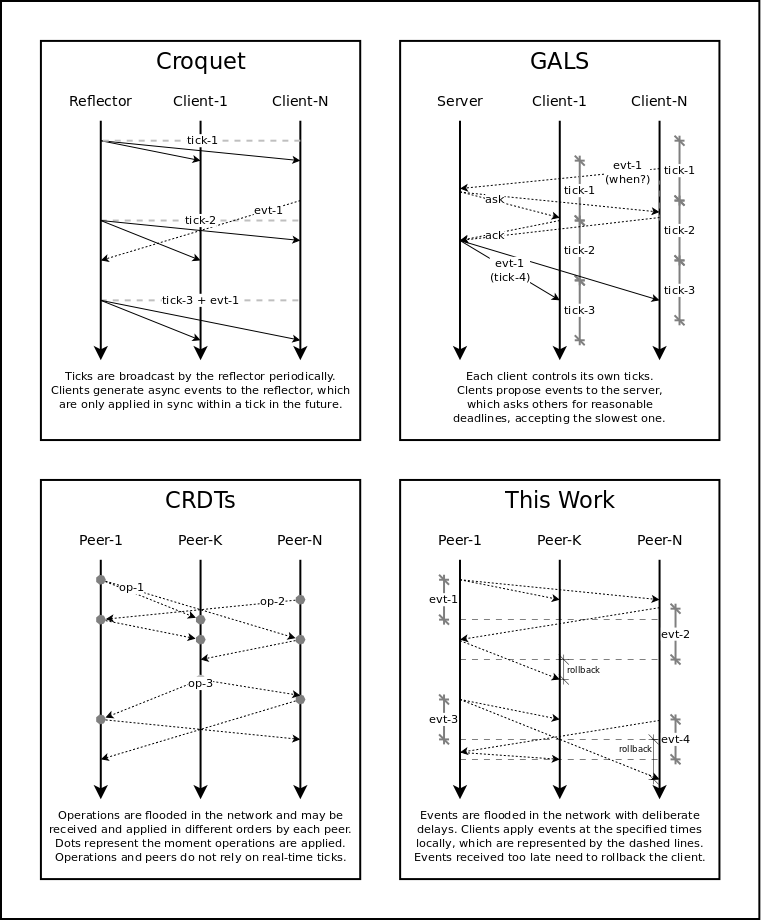
\includegraphics[width=\linewidth]{algos}
  \caption{
    \label{fig.algos}
    Four approaches to symmetric distributed applications: Croquet, GALS,
    CRDTs, and this work.
    The vertical arrows in parallel represent the timelines in nodes in the
    network.
    The arrows crossing nodes represent communication between them.
  }
\end{figure*}

Even though existing solutions aim to provide symmetric behavior for
distributed applications, they diverge in three key aspects as follows:

\textbf{a.} How the network is organized.

\textbf{b.} How global time is determined.

\textbf{c.} How events are propagated and applied.

Figure~\ref{fig.table} compares three selected works regarding these aspects,
which we discuss and contrast with our approach next.
At the end of this section, we also provide initial details on how our
middleware works.

Croquet%
\footnote{Croquet.io: https://croquet.io/}~\cite{croquet} guarantees
bit-identical real-time behavior for users in collaborative distributed
environments.
%
As detailed in Figure~\ref{fig.algos}, a centralized \emph{reflector} issues
periodic ticks, such that all nodes in the network advance together according
to a synchronized global shared clock.
If a user generates an event, it is sent back to the reflector, which
broadcasts the event in the next tick, which all nodes apply in sync.
%
Croquet takes periodic snapshots of the whole application state in order to
support late joins to a running session.
The new node just needs to restore the latest snapshot and simulate the
remaining events to reach the current running state.
%
As indicated in Figure~\ref{fig.table}, Croquet relies on a centralized
network (a), in which nodes advance in sync (b), and in which event outcomes
depend on the central server to be online (c).
%
Note how the central server is the only participant with knowledge about
clients, which never communicate directly among themselves.
This implies that the server must never fail, and also that periodic full
broadcasts are the only possibility of spanning the whole network.
In this work, we argue that in a peer-to-peer alternative any node can fail,
and that broadcasts can be replaced by optimistic flooding.

GALS~\cite{gals} shares the same goals with Croquet, but with some tradeoffs,
mostly favoring clients with slow connections.
As detailed in Figure~\ref{fig.algos}, instead of advancing ticks in sync with
the server, clients have their own independent local clocks.
Event generation requires two round trips (\emph{when → ask → ack → tick}) and is
delayed dynamically according to the slowest client.
%
On the one hand, ticks do not generate any traffic and clients have smooth
frame transitions, even those with poor connections.
On the other hand, events take longer to apply and clients may experience
occasional freezes.
The syncing protocol also requires extra bookkeeping to deal with clock drifts
and client disconnections~\cite{gals}.
%
As indicated in Figure~\ref{fig.table}, GALS also relies on a centralized
network (a), but in which nodes advance time independently (b), and in which
event outcomes still depend on the central server to be online (c).

In both solutions, the network advances together as a whole in real time, with
a total order among events, which is determined by a central server that must
be permanently online.
All clients compute events in sequence, respecting timestamps, and using only
deterministic and stateless calls.
This way, it is guaranteed that all clients reach the same state, and
observe bit-identical steps.

An antagonistic approach to deterministic reactions to events is to model the
application with conflict-free replicated data types~\cite{crdts}.
CRDTs are designed in such a way that all operations are commutative, so that
the order in which they are applied does not affect the final outcome.
%
As detailed in Figure~\ref{fig.algos}, peers can communicate operations
directly to each other with no central authority.
Also, since operations need not to be ordered, they can be applied at the
very first moment they are generated or received, even if the peers are
offline.
%
Since operations must be commutative, it is not possible to timestamp them
in a unique global shared clock.
Hence, there is no notion of a timeline in which peers go through
bit-identical steps, but they do eventually reach the same state.
%
On the one hand, the main advantage of CRDTs is to support local-first
software~\cite{local}, since they can work offline in the same way as online.
On the other hand, they provide very restrictive APIs (the CRDTs themselves),
and do not support real-time consensus among peers.
%
As indicated in Figure~\ref{fig.table}, CRDTs work on decentralized networks
(a), in which peers advance independently (b), and in which operations can be
applied immediately, even while offline (c).
%
Automerge along with its accompanying Hypermerge peer-to-peer infrastructure
is an example of decentralized CRDTs~\cite{p2p.automerge,p2p.pushpin}.

In this work, as indicated in Figure~\ref{fig.table}, our goal is to support
peer-to-peer real-time symmetric execution (a), while still tolerating
out-of-order (b) and offline (c) event generation.
%
As detailed in Figure~\ref{fig.algos}, peers have independent timelines and
can communicate events directly to each other.
Note, that it is not necessary that all peers communicate directly with all
other peers, but only indirectly via unstructured flooding.
Events are delayed to be able to reach other peers in time.
In the case a deadline is missed, the peer rolls back in time and then fast
forwards execution until it catches real-time behavior again.
%
Like Croquet and GALS, peers compute events in sequence using deterministic and
stateless calls only.

Finally, note that classical distributed consensus mechanisms focus on fault
tolerance~\cite{lamport}, but not on real-time symmetric behavior.
These algorithms typically rely on leaders~\cite{consensus.paxos.raft}, which
require an election period that does not cope with our symmetric real-time
requirements.
In this sense, these algorithms could be considered to decentralize servers in
Croquet or GALS, but not to decentralize symmetric peers with high churn rates,
as we propose in this work.
In contrast, our proposal requires a time machine to reapply reordered
operations, since we cannot guarantee strong consistency~\cite{p2p.sec}.

\subsection{Software Time Machines}
\label{sec.related.time}

%We now discuss related work on decentralized and centralized time machines.

A software time machine is a mechanism that allows to regress or advance the
execution of an application.
%
Time travelling is a established research topic for debugging
tools~\cite{tml.review}.
In this context, it is possible to stop a program after a failure and revert
its execution in order to understand the bug causes.
%
In our context of real-time symmetric applications, time travelling is
essential to re-synchronize the execution of mirrored instances that diverge
due to asynchronous events.

Fundamentally, it is not possible to reverse the execution of most programs.
The reason is because even trivial operations, such as `printf` and `abs` are
not invertible.
Therefore, time machines rely on techniques that either \emph{record} the
entire application states in a log, or \emph{reconstruct} them from
deterministic inputs~\cite{tml.review}.
%
In this work, we mix both techniques by taking periodic memory snapshots and
simulating deterministic inputs in between them.

Regarding decentralized machines, Fusion%
\footnote{Fusion: \url{https://doc.photonengine.com/en-us/fusion}}
is a state synchronization networking library for the Unity game engine.
It provides networked tick-based simulation in two modes: client-server
(\emph{hosted mode}) and peer-to-peer (\emph{shared mode}).
The hosted mode is based on continuous memory snapshots, which allows for
full rollbacks when clients diverge.
As discussed in Section~\ref{sec.related.sym}, this approach is similar to how
Croquet handles late joins to a running session.
The shared mode is less powerful and only supports eventual consistency among
clients.
We presume that the reason is because continuous memory snapshots would be too
costly without a central server.

Regarding single-user local machines, the video game Braid%
\footnote{Braid: \url{http://braid-game.com/}}
is designed on the assumption that players have unrestricted rollbacks as part
of the game mechanics.
Like Fusion, the implementation is based on continuous memory snapshots,
instead of deterministic simulation, as we propose in this work.
%
Schuster~\cite{tml.js} proposes a simple API for time travelling in
event-driven JavaScript:
    \code{init()} to return an initial state;
    \code{handle(evt,mem)} to process events and modify state; and
    \code{render(mem)} to output the current state.
As we describe next, we use a similar approach by separating state modification
from rendering~\cite{tml.alive}.

\section{The Middleware \& Programming API}
\label{sec.tml}

The middleware is written in C and relies on the library \emph{SDL}%
\footnote{SDL: \url{http://www.libsdl.org}}
to deal with the network, timers, and input events, such as mouse clicks and
key presses.
The full source code%
\footnote{https://github.com/fsantanna/p2p-tml}
is around 500 lines of code.



\begin{figure}
    \centering
    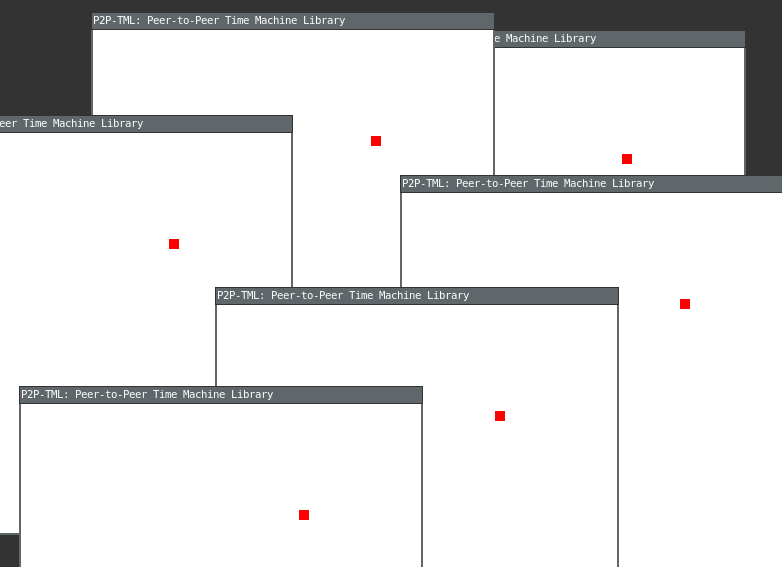
\includegraphics[width=\linewidth]{move}
    \caption[XXX] {
        A moving rectangle is controlled by peers connected indirectly.
        Users can press \code{↑ ↓ → ←} to change the direction of the
        rectangle or \code{SPACE} to pause the application.
        The inputs are applied simultaneously in all peers, as if they were
        mirrors of a single application.
        Video: \url{https://youtu.be/zkl0vSOGino}
        \label{fig.move}
    }
\end{figure}

We guide our discussion through the didactic example of Figure~\ref{fig.move},
in which multiple users use the arrow keys to control the direction of a
moving rectangle.
%
The application is symmetric in the sense that if any user presses a key, a
corresponding event propagates in the network, and all peers apply it
simultaneously, as if they were a single mirrored machine.
At any moment, if a user pauses the application, all peers are guaranteed to
pause exactly at the same frame with the rectangle being ``bit-identically'' at
the same position.

\begin{figure}
  \centering
  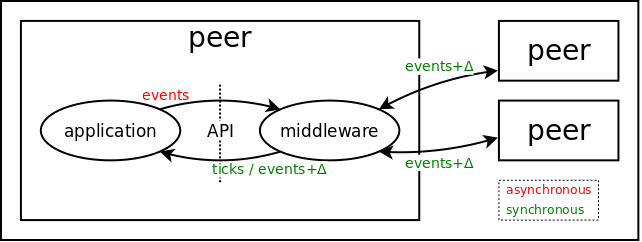
\includegraphics[width=\linewidth]{middleware}
  \caption{
    Applications generate asynchronous events and communicate through an API
    with the middleware.
    The middleware orchestrates the peers, synchronizing their ticks locally
    and disseminating events with a $\Delta$ delay.
    \label{fig.middleware}
  }
\end{figure}

In Figure~\ref{fig.middleware}, a peer is depicted as an application that uses
an API to communicate with the middleware.
The application itself is not aware of the network and has no direct access to
other peers, which communicate transparently through the middleware.
The application generates asynchronous events that go through the middleware,
which synchronizes them with a timestamp with a $\Delta$ delay scheduled to the
future, such that all peers can (optimistically) satisfy.
The middleware controls the execution of the application by issuing ticks and
synchronized events.

The peers form a dynamic unstructured peer-to-peer network~\cite{p2p.survey},
and communicate mostly indirectly to each other.
Events are flooded in the network graph via gossiping, i.e.: when a peer
generates an event, it communicates to its neighbours, which communicate to
their neighbours, and so on.
Note that all peers execute the exactly same application and middleware, with
no differences with respect to their roles and physical resources.
Therefore, we can describe our peer-to-peer network as follows:
    (a) all peers have the same role and run the same software;
    (b) any peer can join or leave at any time;
    (c) events are only communicated with direct neighbours.

The main job of the middleware is to deal with the uncertainties of the
network in order to preserve the symmetric behavior across peers.
As described in the Introduction, the middleware ensures that all peers
    (a) meet event deadlines,
    (b) advance in sync in real time, and
    (c) can leave and join the network and remain symmetric:
%
\begin{enumerate}
\item \textbf{Event Deadlines:}
Due to the inherent latency of networks, peers generate events with a
deliberate delta $\Delta$ so that they can reach other peers in time to be
applied in sync.
%We first assume a predetermined delay for the sake of simplicity.
Nevertheless, a peer ahead of time may receive an event that should have been
applied in the past, even considering the delay.
In this case, the middleware automatically rolls back the peer, applies the
event at the correct time, and then fast forwards the peer, re-applying all
remaining events up to the real time.
As we detail further, rolling back a peer requires to simulate the whole
application execution from the beginning.
As an optimization, the middleware takes periodic snapshots locally at all
peers to avoid full simulation.
%
\item \textbf{Time Synchronization:}
Since peers run in different machines, their timelines will inevitably be out
of sync because applications are launched locally at different times, and
because internal clocks may diverge over time (e.g., from rollbacks or timer
polling inaccuracies).
The middleware assumes the maximum time among all peers to be the
``correct real time'', so that other peers must fast forward to catch up with
it.
Therefore, in order to determine the maximum time and synchronize the clocks,
the middleware proceeds as follows:
    (a) peers disseminate \code{SYNC} events periodically with their local
        times, and
    (b) if a peer is behind a received \code{SYNC}, it advances its frames
        proportionally faster to catch up in time.
%
\item \textbf{Peer Churn:}
Considering that we target peer-to-peer networks, it is important that the
middleware can handle arrival and departure of peers seamlessly.
Note that high churn may lead to intermittent network partitions.
Given our unstructured approach, nothing needs to be done when a peer leaves
the network.
However, when a peer joins the network, the middleware needs to ensure that it
receives from other peer all events that ever happened, in order.
This is trivial since all peers already need to hold the full event history (as
described in item (a)), including their absolute timestamps in the shared
timeline.
In addition, a peer that rejoins the network recovers from a past snapshot it
already holds, thus avoiding full simulation.
\end{enumerate}

\subsection{The Programming API}
\label{sec.tml.api}

The middleware expects to take full control of the application execution in
order to manipulate its timeline and disseminate events in the network.
For this reason, the basic programming API is to call a \code{loop} function
passing a set of callbacks, which the middleware uses to communicate with the
application:

{\footnotesize
\begin{verbatim}
int main (void) {
    p2p_loop (
        1,              // peer identifier
        50,             // simulation FPS
        sizeof(G), &G,  // pre-allocated full state
        cb_ini,         // init/quit callback
        cb_sim,         // simulation callback
        cb_ren,         // rendering callback
        cb_evt          // events callback
    );
}
\end{verbatim}
}

The middleware assumes that each peer assigns itself a unique identifier in a
contiguous range.
The FPS must be the same in all peers to ensure bit-identical simulation.

\subsubsection{Application State}
\label{sec.tml.api.state}

The variable \code{G} passed to the middleware holds the full application
state.
This allows the middleware to take memory snapshots and rollback to previous
states.
If dynamic allocation is required, it is necessary to hold a finite memory
pool in \code{G} with a custom allocator.
In our guiding example of Figure~\ref{fig.move}, the moving rectangle
application only requires to hold the current position and direction:

{\footnotesize
\begin{verbatim}
struct {
    int x,  y;   // position
    int dx, dy;  // direction speed
} G;
\end{verbatim}
}

\subsubsection{Application Events}
\label{sec.tml.api.events}

When an application generates events, they need to propagate in the network
so that all peers behave the same.
Note that application events may (or may not) differ from low-level local
system events.
%which may or may not be mapped 1-to-1 in the callback \code{cb\_evt}.
%
The middleware predefines two events for all applications:
    \code{P2P\_EVT\_START} represents the beginning of the simulation, and
    \code{P2P\_EVT\_TICK} is generated every frame.
The other application-specific events must be declared by the programmer in an
enumeration.
In our example, we define a new event \code{P2P\_EVT\_KEY} to represent key
presses:

{\footnotesize
\begin{verbatim}
enum {
    P2P_EVT_KEY = P2P_EVT_NEXT // next to predefined
};
\end{verbatim}
}

\subsubsection{Initialization Callback}
\label{sec.tml.api.cb_ini}

The middleware calls \code{cb\_ini} twice: at the beginning and at the end of
the loop.
The callback should initialize (and finalize) the network topology, as well as
static immutable globals that can live outside the simulation memory, such as
the window and image textures in our example:

{\footnotesize
\begin{verbatim}
void cb_ini (int ini) {
    if (ini) {
        <...> // create the SDL window
        <...> // open the arrow PNG images
        // create peer links (peer-id, ip, port)
        p2p_link(2, "192.168.1.2", 5000);
    } else {
        <...> // destroy the SDL window
        <...> // destroy the arrow PNG images
        // destroy peer links
        p2p_unlink(2);
    }
}
\end{verbatim}
}

\subsubsection{Simulation Callback}
\label{sec.tml.api.cb_sim}

The middleware calls \code{cb\_sim} every frame or event occurrence, which
should affect the simulation state \code{G} deterministically.
An occurring event may be passed as argument to the callback, which must never
perform any side effects, such as stateful calls or rendering frames.
In our example, we modify the state of the rectangle as follows:
    (a) reset its position and speed on \code{START},
    (b) increment its position based on the current speed on \code{TICK}, and
    (c) modify its speed based on \code{KEY}:

{\footnotesize
\begin{verbatim}
void cb_sim (p2p_evt evt) {
    switch (evt.id) {
        case P2P_EVT_START: // resets pos and speed
            G.x = G.y = G.dx = G.dy = 0;
            break;
        case P2P_EVT_TICK:  // increases position
            G.x += G.dx * VEL;
            G.y += G.dy * VEL;
            break;
        case P2P_EVT_KEY:   // modifies speed
            switch (evt.pay.i1) {
                case SDLK_UP:
                    G.dx = 0;
                    G.dy = -1;
                    break;
                <...> // same for other keys
            }
            break;
    }
}
\end{verbatim}
}

The calls to \code{cb\_sim} normally happen during real-time simulation, i.e.,
while the user is interacting with the application.
However, if the peer is out of sync, the middleware may ``time travel'' and
call the simulation many times to go back and forth and catch up with real
time.
This is the reason why we define \code{START} as an event like any other:
travelling requires to simulate the execution from the beginning, event by
event.

\subsubsection{Rendering Callback}
\label{sec.tml.api.cb_ren}

Time travelling is also the reason why \code{cb\_sim} must be separated from
the rendering callback \code{cb\_ren}~\cite{tml.js}, which would otherwise
render the screen multiple times while travelling.
%, which the middleware calls only on real-time frames.
In our example, \code{cb\_ren} just needs to redraw the rectangle at the
current position:

{\footnotesize
\begin{verbatim}
void cb_ren (void) {
    <...> // clears the SDL window
    // redraws the rectangle at the current position
    SDL_Rect r = { G.x, G.y, 20, 20 };
    SDL_DrawRect(&r);
}
\end{verbatim}
}

\subsubsection{Events Callback}
\label{sec.tml.api.cb_evt}

The callback \code{cb\_evt} is called by the middleware in real time, whenever
a local SDL event occurs.
This callback has two goals:
    (a) map and propagate application events, and
    (b) provide instant feedback to the user.
%As mentioned previously,
Not all local low-level events need to correspond to application events in the
network.
The callback is allowed to perform side effects, such as modifying the network
topology, or exhibiting instant feedback on the screen.
In our example, we only generate application events for the 5 key events of
interest, but we also exhibit the pressed key in real time as a visual
feedback:

{\footnotesize
\begin{verbatim}
int cb_evt (SDL_Event* sdl, p2p_evt* evt) {
    if (sdl->type == SDL_KEYDOWN) {
        if (sdl->key == <any-of-the-keys>) {
            SDL_DrawImage(<img-of-the-key>);
            *evt = (p2p_evt){ P2P_EVT_KEY,sdl->key };
            return 1; // generate application event
        }
    }
    return 0; // otherwise, do not generate any event
}
\end{verbatim}
}

\subsection{Middleware Orchestration}
\label{sec.tml.middleware}

We now detail how the middleware orchestrates an application and ensures that
all peers
    (a) meet event deadlines,
    (b) advance in sync in real time, and
    (c) can leave and join the network and remain symmetric.

\subsubsection{Event Dissemination}
\label{sec.tml.middleware.events}

As illustrated in Figure~\ref{fig.middleware}, events propagate between peers
with a timestamp scheduled to the future with an extra delta $\Delta$ such that
all peers are able to apply them in sync.
%
To prevent dissemination cycles, each peer keeps a vector with the highest
timestamp it received from each other peer, such that lower numbers can be
ignored when received.
Since we rely on TCP connections, it is not possible to receive out-of-order
timestamps attached to a given source peer.
When the middleware receives a higher number from a given peer, it updates its
vector position and triggers an event propagation to neighbours.
%
As mentioned in Section~\ref{sec.tml.api}, we assume that peers assign
themselves unique identifiers in a contiguous range, such that they fit in a
simple vector of timestamps.

When receiving an unseen event, the middleware also enqueues it in timestamp
order and calls the application callback \code{cb\_sim} at the appropriate
time.
Peers must keep the full event queue in memory for two reasons:
    (a) receiving a late event may reorder it and require a time travel, and
    (b) peers that join the network need to receive all events.
%
Therefore, the middleware keeps a queue of ``packets'', which includes the
event and additional metadata:

{\footnotesize
\begin{verbatim}
typedef struct {
    uint8_t  src;       // source peer
    uint32_t tick;      // tick to apply
    p2p_evt  evt;       // event id + payload
} p2p_pak;

struct {
    int i;  // next event to apply in real time
    int n;  // number of events in the queue
    p2p_pak buf[MAX];   // queue of packets
} PAKS;
\end{verbatim}
}

Considering the peer-to-peer network as a whole, each event packet is
replicated to all neighbours of all peers.
This results in a theoretical limit of quadratic messages if all peers were
connected to all peers.
In contrast, as discussed in Section~\ref{sec.related.sym}, a centralized
solution only requires a packet to be sent to a server, which then broadcasts
it to all clients.

\subsubsection{The Main Loop}
\label{sec.tml.middleware.loop}

The middleware main loop \code{p2p\_loop} is responsible for calling the
application callbacks, and also controlling its timeline.
The loop continuously checks for network packets, local inputs, and time ticks,
as follows:

{\footnotesize
\begin{verbatim}
01  void p2p_loop (...,cb_ini,cb_sim,cb_ren,cb_evt) {
02    cb_ini(1);    // initialization
03    cb_sim(<P2P_EVT_START>);
04
05    while (<app-running>) {
06      if (<next-network-packet>) {
07        // fast forward if I'm late
08        if (<packet-sync-future>) {
09          p2p_travel(<now>, <pak-sync-time>, <vel>);
10        }
11
12        // travel back & forth if I'm early
13        if (<packet-evt-past>) {
14          p2p_travel(<now>, <pak-evt-time>, <vel>);
15          p2p_travel(<pak-evt-time>, <now>, <vel>);
16        }
17
18        // real time if I'm on time
19        if (<packet-evt-ok>) {
20          cb_sim(<packet-evt>);
21          cb_ren();
22        }
23      }
24
25      if (<next-local-input>) {
26        // propagate local event
27        p2p_evt evt;
28        if (cb_evt(&evt)) {
29          p2p_propagate(<future>, &evt);
30        }
31      }
32
33      // simulate tick in real time
34      if (<next-local-tick>) {
35        cb_sim(<P2P_EVT_TICK>);
36        <application-snapshot-every-second>
37        cb_ren();
38      }
39    }
40
41    cb_ini(0);    // finalization
42  }
\end{verbatim}
}

The function receives the application callbacks as arguments \lin{1}
(Section~\ref{sec.tml.api}).
We first (and last) call \code{cb\_ini} to initialize (and finalize) the
application \lin{2,41}.
Then, we call \code{cb\_sim} \lin{3}, passing the event \code{START} to start
the application in real time
(Sections~\ref{sec.tml.api.events}~and~\ref{sec.tml.api.cb_sim}).
The main loop \lin{5--39} checks continuously for network packets \lin{6--23},
local input events \lin{25--31}, and time ticks \lin{33--38}.

Regarding network packets, if we receive a time synchronization packet
\code{SYNC} from the future \lin{7--10}, then we fast forward the application
to catch up in time (Section~\ref{sec.tml}.b).
If we receive an event that should have been applied in the past \lin{12--16},
then we travel back and forth (Section~\ref{sec.tml}.a).
Otherwise, we just apply the event in real time \lin{18--22}
(Section~\ref{sec.tml.api.cb_sim}).
We detail the function \code{p2p\_travel} in
Section~\ref{sec.tml.middleware.travel}.
%
Regarding local inputs, we call \code{cb\_evt} to signal if the event should be
disseminated \lin{26--30}, also transforming it into an application event
(Section~\ref{sec.tml.api.cb_evt}).
%
Regarding time ticks, we call \code{cb\_sim} and \code{cb\_ren} in real time
\lin{33--38}.
The middleware also takes periodic snapshots of the application state to
optimize time travelling (Section~\ref{sec.tml.api.state}).

\subsubsection{The Time Machine}
\label{sec.tml.middleware.travel}

The last important mechanism of the middleware is the time machine, which
allows to move the application back and forth in time:

{\footnotesize
\begin{verbatim}
01  void p2p_travel (int from, int to, int ms) {
02    for (i=from..to) {
03      int bef = <tick-of-snapshot-before-i>
04      <restore-snapshot-at-bef>
05      for (j=bef..i) {
06        cb_sim(<tick-or-evt-at-j>)
07      }
08      cb_ren();
09      <delay-ms>
10    }
11  }
\end{verbatim}
}

The function \code{p2p\_travel} time travels the application, starting at tick
\code{from}, tick by tick \lin{2--10}, until it reaches tick \code{to}.
The loop can travel in both directions, i.e., \code{from} may be higher than
\code{to}.
At each step, we need to find the tick \code{bef} with the closest past
snapshot \lin{3}, restore it \lin{4}, and than simulate the remaining steps
from the snapshot to the desired tick \lin{5--7}.
We also exhibit each step with a small \code{ms} delay \lin{8--9} so that users
experience smooth time transitions.

The step delay is dynamically adjusted such that the whole time travel loop
takes at most 1 second to complete.
Note that during this period, the application is frozen, and new inputs are
enqueued for further processing.

\subsubsection{Middleware Summary}
\label{sec.tml.middleware.summary}

This section provided an overview of the middleware implementation to answer
how it ensures the desired properties in concrete terms as follows:
    (a) peers meet event deadlines either travelling back and forth or in real
        time (\linx{12--16} or \lin{18--22} / \ref{sec.tml.middleware.loop});
    (b) peers synchronize their clocks with periodic \code{SYNC} packets that
        fast forward late peers
        (\linx{7--10} / \ref{sec.tml.middleware.loop}); and
    (c) peers can join the network at any time and still catch up in time by
        receiving the full event history
        (Section~\ref{sec.tml.middleware.events}).

As discussed in Section~\ref{sec.tml.api}, the middleware imposes some
restrictions, which are discussed as follows:

\begin{itemize}
%
\item \textbf{Contiguous unique identifiers:}
We assume that peers have unique identifiers in a contiguous range, which
allows us to hold the peers database in a vector.
Nevertheless, it is possible to generate UUIDs based local information
only~\cite{p2p.id}, and to use a hash table as database instead.
%
\item \textbf{Deterministic API:}
Since simulations must be equally reproduced in all peers, non-deterministic
APIs are forbidden.
This is a fundamental limitation that cannot be easily overcame.
Note that the alternatives discussed in Section~\ref{sec.related} either impose
the same limitation~\cite{croquet,gals}, or can be even more restrictive
allowing only CRDTs~\cite{crdts}.
%
\item \textbf{Non-malicious peers:}
As detailed in Section~\ref{sec.tml.api.cb_evt}, note that the API to
disseminate an event in the network is as simple as a variable assignment.
Therefore, a malicious peer could SPAM or inject erroneous events to break the
application.
Again, this is a fundamental limitation that is also shared with the
alternatives discussed in Section~\ref{sec.related}.
%
\item \textbf{Static memory footprint:}
The middleware takes periodic snapshots of the whole application state in order
to optimize time machine simulations and resynchronize peers.
This mechanism imposes two challenges:
first, the snapshot must be small and determined, which implies a contiguous
static region;
second, the history of snapshots must be stored in all peers.
Currently, we allocate periodic snapshots assuming that the memory does not
deplete until the application terminates.
Alternative policies could favor recent snapshots or simply impose a limit that
reject clients that are too late.
Regarding the static limitation, we mentioned the possibility of a custom
allocator, which is illustrated as follows:
\end{itemize}

{\footnotesize
\begin{verbatim}
struct {
    // FIXED REGION
    int x,  y;   // position
    int dx, dy;  // direction speed
    // VARIABLE REGION
    char heap[HEAP_SIZE];
} G;

T* obj = my_malloc(G.heap, <size>);
<...>
my_free(obj);
\end{verbatim}
}

The variable region is still technically static, but is dynamically reshaped
internally with the custom allocator \code{my\_alloc} \& \code{my\_free}.

%\newpage
\section{Evaluation}
\label{sec.eval}

In this section, we evaluate if our design meets the goals to ensure that all
peers
    (a) meet event deadlines,
    (b) advance in sync in real time, and
    (c) can leave and join the network and remain symmetric.
%
We perform simulations varying the network latency and peer churn, as well as
the frequency and deadlines of events.
%
We then measure
    (a) the recurrence of time travels,
    (b) the real-time pace of peers, and
    (c) the recoverability from churns,
such that they validate our goals above, respectively.

Regarding (a), if a peer experiences a time travel, it means that it received
an event after its deadline.
We then count all time travel occurrences in our evaluation.
%
Regarding (b), we use an absolute simulation clock to track, in real time, the
execution pace of each peer.
% in comparison to the reference peer, which is the one most advanced in time.
We then count the mismatches between the clocks in our evaluation.
%
Regarding (c), we make peers leave and join the network periodically, possibly
creating partitions.
We then assert that they all catch up in real time within a short period in our
evaluation.

\begin{figure*}
  \centering
  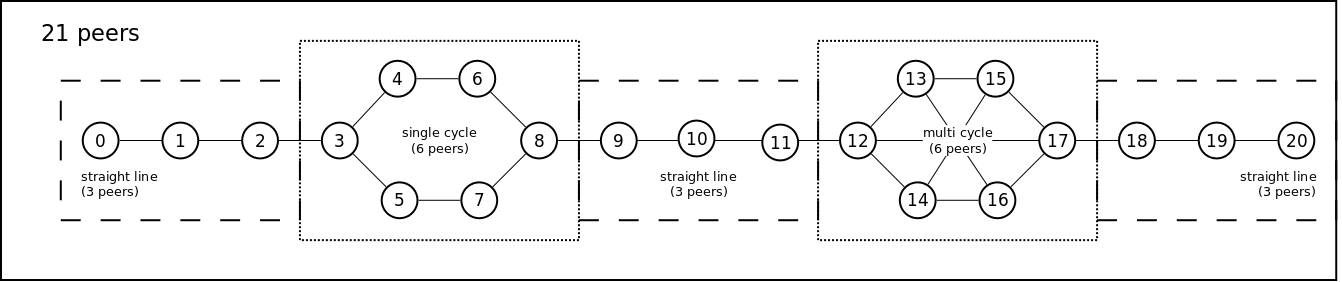
\includegraphics[width=\linewidth]{topo}
  \caption{
    \label{fig.topo}
    Network topology: 21 peers organized as a straight line ($0-3$), a simple
    cycle ($3-8$), a second straight line ($8-11$), a full connected cycle
    ($12-17$), and a third straight line ($17-20$).
    %An optional link ($0,20$) creates a long cycle in the network.
  }
\end{figure*}

\begin{figure}
  \centering
  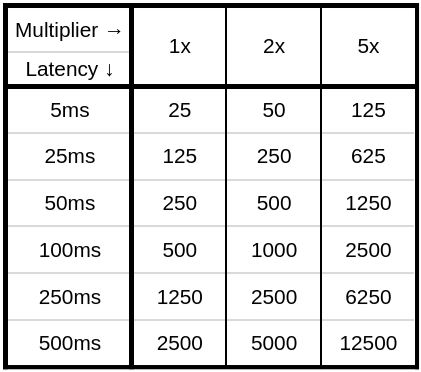
\includegraphics[width=2in]{mult}
  \caption{
    \label{fig.mult}
Event delays in $ms$ considering the network latency, delay multiplier, and the
average of 5 hops between peers from Figure~\ref{fig.topo}.
    }
\end{figure}

We perform simulations with 21 peers using the mixed topology of
Figure~\ref{fig.topo}, with peers organized in straight lines and cycles.
The topology has an average of 5 hops between peers (e.g., \code{4-16} are 7
hops away).
%
We run the application main loop at $50~FPS$ ($20ms$ per frame) and calculate
the middleware overhead at each iteration, which is $9us$ in the average,
corresponding to less than $1/2000$ of the CPU time.
%
In order to have an absolute clock, we use a single machine to simulate all
peers, allowing us to merge their logs into a single file with a comparable
shared timeline.
%
We use \emph{NetEm}~\cite{netem} to simulate the network latency with a normal
distribution.
% (e.g., \code{tc qdisc add dev lo root netem delay 200ms 40ms distribution normal}).
%
We vary
    (i)   the network latency ($5-500ms$ between each peer),
    (ii)  the rate of events ($5-200~evt/sec$), and
    (iii) the delay multiplier ($1-5x$).
%
Figure~\ref{fig.mult} shows the event delays considering the network latency
and chosen multiplier.
For instance, a $50ms$ latency with a $2x$ multiplier results in $500ms$ event
delays, i.e., each event is triggered with this delay to compensate the given
latency and fixed average of 5 hops.
%
These variations result in $108$ combinations.
We executed each combination $3$ times for $5$ minutes each.
We also make some modifications to evaluate peer churn, which requires to
re-execute the simulation.
The experiments take around $40$ hours to complete.

% https://docs.google.com/spreadsheets/d/1xK5_wF9MoR-SmPGWVj0sGLrHxhpPBlLjVoS8U-Y7zTQ/edit#gid=63016757

\begin{figure*}
  \centering
  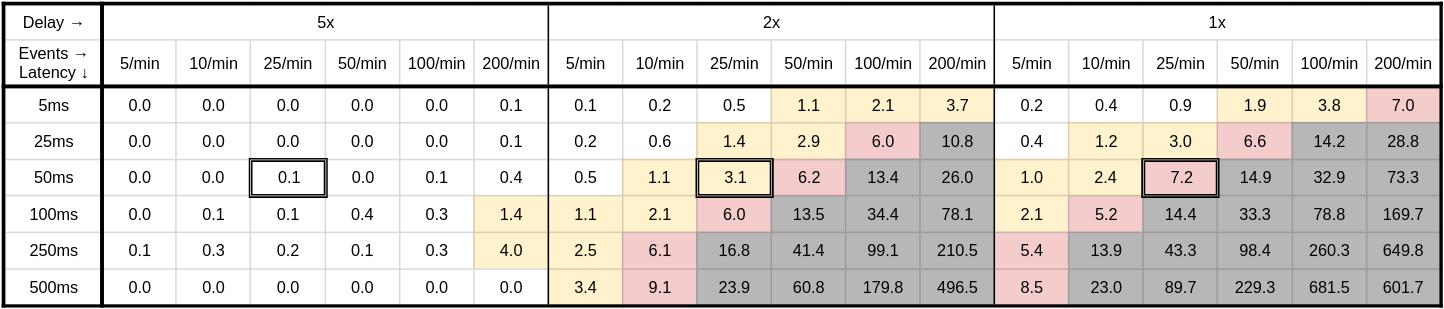
\includegraphics[width=\linewidth]{baks}
  \caption{
    \label{fig.baks}
The $5x$, $2x$, and $x$ delay regions each contains $36$ measures for multiple
configurations of event rate ($5-200~evt/min$ and network latency ($5-500ms$).
%
The color thresholds (\emph{white}, \emph{yellow}, \emph{red}, \emph{black})
are arbitrary but help to distinguish between regions of interest.
%
The experiments uses $1$ process for each peer in a single Linux machine
(\emph{i7/16GB}).
    }
\end{figure*}

We now detail the results and how we instrument the middleware implementation
to measure the properties above:

\textbf{(a) Recurrence of time travels:}
Every time a peer is ahead in time and needs to travel back, we output its id
and how much ticks it needs to travel back.
At the end, we measure the percentage of the sum of all time travel ticks over
the total simulation ticks.
As an example, if all peers sum $1000$ time travel ticks over $100k$
accumulated simulation ticks, then the final measure is $1\%$.
%
Figure~\ref{fig.baks} presents the results considering all combinations of
parameters (i), (ii), and (iii) above.
The colors indicate the feasibility of each tested scenario
    (\emph{white=good}, \emph{yellow=moderate}, \emph{red=poor},
    \emph{black=faulty}).
%
For instance, the three framed rectangles ($0.1$, $3.1$, and $7.2$) in the
figure represent the scenarios with $50ms$ network delay, generating
$25~evt/min$.
Each rectangle uses a different delay multiplier, showing a good performance
for $5x$, moderate for $2x$, and poor for $1x$.

\textbf{(b) Real-time pace of peers:}
All peers output their current ticks continuously, allowing us to compare them
in the shared timeline.
Every time we see a greater tick never seen in the timeline before, we count
smaller ticks from other peers, which constitute time violations.
As an example, if all peers sum $1000$ of such smaller ticks over $100k$
accumulated simulation ticks, then the final measure is $1\%$.
%
We also start each peer with a random delay of up to $10s$ to force a
synchronization mismatch at the beginning.
%
Considering all scenarios, the average is negligibly under $0.2\%$, with no
significant variance.
Therefore, we omit the resulting table akin to Figure~\ref{fig.baks}), which
would not provide further insights.

\textbf{(c) Correctness of unstable peers:}
We tweak our simulation to make each peer remain $40s$ online and $20s$
offline in the average, including peers \code{9-11} in the middle of the
network.
This creates partitions in the network, which generate events out of sync that
require constant resynchronization between peers.
%
Then, to evaluate the network correctness under such high churn, we count how
much time a recovering peer takes to catch up in real time:
When a peer becomes online, we take the current maximum tick considering all
reachable peers, and then count the time the recovering peer takes to catch up.
We also assert that they all reach the same final state eventually.
%
Considering all scenarios, the average is $1.3$ seconds of recovering time,
with no significant variance.
Therefore, we also omit the resulting table (akin to Figure~\ref{fig.baks}).

Our results show that goals (b) and (c) are met in all scenarios consistently,
and we consider them nearly optimal:
Regardless of the network latency, event rate, and delay multiplier,
    the variation in the pace of peers is under $0.2\%$ (goal b), while
    recovering peers take $1.3$ seconds to catch up in time (goal c).
Note that the middleware makes smooth time transitions in small steps that take
$1$ second to complete, resulting in no more than 2 time travels to recover
peers.

Considering goal (a), we need to take a closer look at Figure~\ref{fig.baks}.
The color patterns indicate clear boundaries for the scenarios that can meet
event deadlines with the desired performance.
%
For instance, high event delays (column $5x$) make all scenarios viable,
even with high latency and event frequency.
As an application example, chats are not affected by high event delays.
Nevertheless, the higher are the event delays, the less applications suit the
middleware.
%
For the lowest possible delay (column $1x$), we see that the middleware can
either handle low latency with high event frequency (e.g., $5ms$ with
$100evt/min$) or high latency with low event frequency (e.g., $100ms$ with
$5evt/min$).
%
The color patterns in the table provide the necessary information to confront
an application with its feasibility or desired performance.

Considering the metrics we evaluate, we now compare our work with the existing
solutions of Section~\ref{sec.related.sym}:

\textbf{(a) Recurrence of time travels:}
In Croquet, the centralized reflector issues periodic ticks, which represents
the only authority over time.
On the one hand, clients never need to travel back in time, but on the other
hand, the reflector represents a single point of failure.
%
GALS imposes the same tradeoffs, relying on a central server to provide a
single authority over time.
%
CRDT operations can be applied in any order, which also excludes time travels
entirely.
However, the notion of a shared real-time timeline cannot exist, which
precludes bit-identical behavior across peers.

\textbf{(b) Real-time pace of peers:}
Croquet stipulates a global tick period which all clients must comply with.
However, clients with poor connections experience constant freezes and cannot
advance in real time.
As a concrete example, a peer that experiences a latency of $500ms$, while the
reflector issues ticks every $100ms$, will freeze for $400ms$, even if no
events occur in the network.
%
GALS supports independent timelines for clients, but at the cost of applying
events with a greater delay in comparison to Croquet.
%
With CRDTs, although peers advance independently, the notion of real time does
not exist.

\textbf{(c) Correctness of unstable peers:}
Since clients are connected directly with the server, Croquet and GALS have no
issues with unstable clients.
When reconnecting, a client just needs to synchronize pending events from the
server and apply them in order.
However, as discussed before, the server represents a single point of failure.
%
CRDTs are also immune to unstable peers, since peers just need to synchronize
events and apply them in any order, but again missing the notion of real-time
behavior.

\section{Conclusion}
\label{sec.conclusion}

We propose a middleware to program \emph{symmetric peer-to-peer applications}
in which interacting decentralized instances conform to identical behavior.
%
The middleware API shares similar limitations with centralized
alternatives~\cite{gals,croquet}, being restricted to deterministic and
stateless calls, and only supports pre-allocated memory.
%
Our main contribution is a ``time machine'' based on memory snapshots and
deterministic simulation, allowing to decentralize the network timeline such
that conflicting peers can rollback and resynchronize their state.
%
We assume that peers are non-malicious and that they can assign themselves
unique identifiers in a contiguous range.

The middleware can handle applications with over 20 peers in a heterogeneous
topology under high churn.
%
We show that peers can
    (a) disseminate events and meet deadlines globally, 
    (b) advance in sync in real time, and
    (c) leave and join the network and remain symmetric.
%
In our experiments, we vary the network latency and the rate and deadline of
events.
We than measure the recurrence of time travels in the network as a
representative of quality.
%
As a result, we present a feasibility table to indicate the application
scenarios that the middleware can handle.
For instance, in a simulation scenario of 25 events per minute with a network
latency of $50ms$, the peers need to roll back and resynchronize only $3\%$ of
the time.

%----------------------------------------------------------------------------------------
%	REFERENCE LIST
%----------------------------------------------------------------------------------------

\phantomsection


\makeatletter
\renewcommand\@biblabel[1]{{\parbox{0.7cm}{[#1]}}}
\makeatother
% References
\renewcommand{\refname}{References}
\bibliography{rita}

\balance
\end{document}
